%%%%%%%%%%%%%%%%%%%%%%%%%%%%%%%%%%%%%%%%%%%%%%%%%%%%%%%%%%          METAPODATKI

\begin{filecontents*}{\jobname.xmpdata}
\Title{Naslov magistrskega dela}
\Author{Ime in priimek}
\Keywords{magisterij\sep navodila\sep ključne besede}
\Publisher{Univerza v Ljubljani, Fakulteta za matematiko in fiziko}
\end{filecontents*}

%%%%%%%%%%%%%%%%%%%%%%%%%%%%%%%%%%%%%%%%%%%%%%%%%%%%%%%%%%

\documentclass[longbibliography,slovene,a4paper,12pt]{book}
%\usepackage[english]{babel}    % angleski delilni vzorci
\usepackage[slovene]{babel}    % slovenski delilni vzorci
\usepackage[utf8]{inputenc}
\usepackage{amsfonts}
\usepackage[T1]{fontenc}
\usepackage[pdftex]{graphicx}
\usepackage{fancyhdr}
\usepackage[sort, numbers]{natbib}
\setlength{\parindent}{0pt}%ni pomika za paragrafe
\setlength{\parskip}{0.75ex}%med paragrafi je malo lufta

\usepackage[pdftex]{graphicx}%za slike: predvidimo da bomo klicali pdflatex.

\usepackage{amsmath}
\usepackage{amsfonts}
\usepackage{mathrsfs}
\usepackage[usenames]{color}
\usepackage[slovene]{babel}
\usepackage[utf8]{inputenc}%to omogoca uporabo sumnikov. Brez tega rabis \v{c}, \v{s}, \v{z} in vse ostalo.

%nekaj koristnih funkcij.
\newcommand{\HRule}{\rule{\linewidth}{0.5mm}}   %debela črta čez celo stran

\newcommand{\ve}[1]{\ensuremath{\mathbf{#1}}} % for vectors
\newcommand{\gv}[1]{\ensuremath{\mbox{\boldmath$ #1 $}}} 
% for vectors of Greek letters
\newcommand{\uv}[1]{\ensuremath{\mathbf{\hat{#1}}}} % for unit vector
\newcommand{\abs}[1]{\left| #1 \right|} % for absolute value

\renewcommand{\Re}{\mathop{\rm Re}}
\renewcommand{\Im}{\mathop{\rm Im}}
\newcommand{\Tr}{\mathop{\rm Tr}}
\newcommand{\dd}{\,\mathrm{d}}
\newcommand{\ddd}{\mathrm{d}}
\newcommand{\ii}{\mathrm{i}}
\newcommand{\lag}{\mathcal{L}\!}
\newcommand{\ham}{\mathcal{H}\!}
\newcommand{\four}[1]{\mathcal{F}\!\left(#1\right)}
\newcommand{\bigO}[1]{\mathcal{O}\!\left(#1\right)}
\newcommand{\sh}{\mathop{\rm sinh}}
\newcommand{\ch}{\mathop{\rm cosh}}
\renewcommand{\th}{\mathop{\rm tanh}}
\newcommand{\erf}{\mathop{\rm erf}}
\newcommand{\erfc}{\mathop{\rm erfc}}
\newcommand{\sinc}{\mathop{\rm sinc}}
\newcommand{\rect}{\mathop{\rm rect}}
\newcommand{\ee}[1]{\cdot 10^{#1}}
\newcommand{\inv}[1]{\left(#1\right)^{-1}}
\newcommand{\invf}[1]{\frac{1}{#1}}
\newcommand{\sqr}[1]{\left(#1\right)^2}
\newcommand{\half}{\frac{1}{2}}
\newcommand{\thalf}{\tfrac{1}{2}}
\newcommand{\pd}{\partial}
\newcommand{\Dd}[3][{}]{\frac{\ddd^{#1} #2}{\ddd #3^{#1}}}
\newcommand{\DD}[3][{}]{\frac{D^{#1} #2}{D #3^{#1}}}
\newcommand{\Pd}[3][{}]{\frac{\pd^{#1} #2}{\pd #3^{#1}}}
\newcommand{\bra}[1]{\langle #1 \vert}
\newcommand{\ket}[1]{\vert#1\rangle}
\newcommand{\avg}[1]{\left\langle#1\right\rangle}
\newcommand{\norm}[1]{\left\Vert #1 \right\Vert}
\newcommand{\braket}[2]{\left\langle #1 \vert#2 \right\rangle}
\newcommand{\obraket}[3]{\left\langle #1 \vert #2 \vert #3 \right \rangle}
\newcommand{\en}[1]{\mathop{\rm #1}}
\newcommand{\hex}[1]{\texttt{0x#1}}

\renewcommand{\iint}{\mathop{\int\mkern-13mu\int}}
\renewcommand{\iiint}{\mathop{\int\mkern-13mu\int\mkern-13mu\int}}
\newcommand{\oiint}{\mathop{{\int\mkern-15mu\int}\mkern-21mu\raisebox{0.3ex}{$\bigcirc$}}}

\newcommand{\wunderbrace}[2]{\vphantom{#1}\smash{\underbrace{#1}_{#2}}}


\renewcommand{\vec}[1]{\overset{\smash{\hbox{\raise -0.42ex\hbox{$\scriptscriptstyle\rightharpoonup$}}}}{#1}}
\newcommand{\bec}[1]{\mathbf{#1}}

%\pagestyle{plain}
\pagestyle{headings}


%%%%%%%%%%%%%%%%%%%%%%%%%%%%%%%%%%%%%%%%%%%%%%%%%%%%%%%%%%       PDF/A

\usepackage{xmpincl}
\usepackage[a-1b]{pdfx}       

%%%%%%%%%%%%%%%%%%%%%%%%%%%%%%%%%%%%%%%%%%%%%%%%%%%%%%%%%%

\usepackage{hyperref}
\usepackage[a4paper,inner=3.5cm,outer=2.5cm,top=2.5cm,bottom=2.5cm,pdftex]{geometry}
\usepackage[titletoc,title]{appendix}
\usepackage{epstopdf}
\usepackage{url}
\usepackage{makeidx}
\pagestyle{headings}
\makeindex

%%
%% Za pisanje sumnikov imamo tri moznosti:
%%   --- vnasamo jih neposredno v kodnem sistemu UTF-8 
%%   --- pisemo jih z latexovim ukazom, ki je namenjen natanko temu,
%%       in sicer kot \v{c}, \v{s}, \v{z}, \v{C}, \v{S}, v{\Z} ali
%%       malo manj pregledno kot \v c, \v s, \v z, \v C, \v S, \v Z,
%%   --- pisemo jih kot "c, "s, "z, "C, "S, "Z), vendar tedaj potrebujemo
%%       spodaj zapisani macro, ki znaku " pripise vlogo `izdelave' sumnika:
% \catcode`\"=\active\def"#1{\v{#1}}
%%       torej \v{S}krjan\v{c}ek == \v Skrjan\v cek == "Skrjan"cek
%% Pozor: narekovaj potem ne smemo vec pisati kot " ampak kot `` in '',
%%       torej: "Skrjan"cek je "civkal ``"ci-"ci-"ci''.

%%
%% Mozni nacini stevilcenja strani:
%%  --- arabske stevilke v celotnem dokumentu, kot je uporabljeno v tej predlogi
%%  --- del strani je lahko stevilcen z rimskimi stevilkami, razen uvoda, osrednjega dela, zakljucka in seznama literature.
%% V vsakem primeru se stevilke na straneh izpisejo sele od kazala naprej.

\def\epsfg#1#2{\epsfig{file=#1.eps,width=#2}}
\def\legendamp#1#2{\vbox{\hsize=#1\caption{\small #2}}}

\setcounter{topnumber}{4}
\setcounter{bottomnumber}{4}
\setcounter{totalnumber}{5}
\renewcommand{\topfraction}{0.99}
\renewcommand{\bottomfraction}{0.99}
\renewcommand{\textfraction}{0.0}
\setlength{\tabcolsep}{10pt}
\renewcommand{\arraystretch}{1.5}

\def\bi#1{\hbox{\boldmath{$#1$}}}
\let\oldvec\vec
\def\vec#1{\mbox{\boldmath$#1$}}
\def\pol{{\textstyle{1\over2}}}
\def\svec#1{\mbox{{\scriptsize \boldmath$#1$}}}

\begin{document}

%%% NASLOVNA STRAN

\pagestyle{empty}
\begin{center}

{\large UNIVERZA V LJUBLJANI\\
FAKULTETA ZA MATEMATIKO IN FIZIKO\\
ODDELEK ZA FIZIKO\\
PROGRAM in SMER ŠTUDIJA\\}


\vspace{4cm}


{\Large Ime in priimek\\}

\vspace{10mm}

{\bf \Large NASLOV MAGISTRSKEGA DELA}\\
\vspace{5mm}
{\large Magistrsko delo}\\




\vfill



{\large MENTOR$\backslash$-ICA: naziv, Ime in priimek\\
SOMENTOR$\backslash$-ICA: naziv, Ime in priimek\\


\vspace{2cm}
Ljubljana, leto}

\end{center}

%%% ZAHVALA (NEOBVEZNO)

\cleardoublepage
\mbox{}
\vfill
{\Large \bf Zahvala}
\vspace{1cm}\\

%%% IZVLECEK

\cleardoublepage
{\Large \bf Izvleček}
\vspace{1cm}\\
Kratek izvleček v slovenskem jeziku.\\
\vspace{1cm}\\
{\bf Ključne besede:}\\
{\bf PACS:}

%%% ABSTRACT

\cleardoublepage
{\Large \bf Abstract}
\vspace{1cm}\\
Kratek izvleček v angleškem jeziku.
\vspace{1cm}\\
{\bf Keywords:}\\
{\bf PACS:}

%%% KAZALO

\tableofcontents

%%% SEZNAM SLIK (NEOBVEZNO)

\cleardoublepage\phantomsection
\renewcommand\listfigurename{Seznam slik}
\addcontentsline{toc}{chapter}{\listfigurename}
\listoffigures

%%% SEZNAM TABEL (NEOBVEZNO)

\cleardoublepage\phantomsection
\renewcommand\listtablename{Seznam tabel}
\addcontentsline{toc}{chapter}{\listtablename}
\listoftables

\cleardoublepage

%%% OSREDNJI DEL

\pagestyle{fancy}
\fancyhead[CE,RE]{}
\fancyhead[LO,CO]{}
\fancyhead[LE]{\textbf{\nouppercase{\leftmark}}}
\fancyhead[RO]{\textbf{\nouppercase{\rightmark}}}

%\include{Uvod}

\chapter{Uvod}
\label{ch1}

\index{BibTeX}

N
%\include{Matemati"cni izrazi}

\chapter{Matematični izrazi}
\label{ch2}



\section{Osnovne enačbe gibanja}
\subsection{Newtonovi zakoni}





%\include{Slike in tabele}

\chapter{Slike in tabele}
\label{ch3}

% Slike in dalj"se tabele praviloma vklju"cujemo v dokument kot 
% plavajo"ce objekte ali plovke (angle"sko floats).
% Polo"zaj plovke v kon"cnem izdelku je odvisen od poteka besedila.
% "Ce "zelimo dolo"citi to"cno mesto plovke, ukazu \verb|\begin{figure}|
% ali \verb|\begin{table}| dodamo [dolo"cilo]:

\begin{itemize}
\item[---]{{\tt h} \hspace{1 cm} tukaj}
\item[---]{{\tt t} \hspace{1 cm} na vrhu strani}
\item[---]{{\tt b} \hspace{1 cm} na dnu strani}
\item[---]{{\tt p} \hspace{1 cm} na posebni strani}
\end{itemize}

\noindent
Slike in tabele potrebujejo podnapise s pojasnili. Vkolikor je slika povzeta iz drugega vira, mora biti tudi ta naveden:

% \begin{figure}[h]
% \begin{center}
% 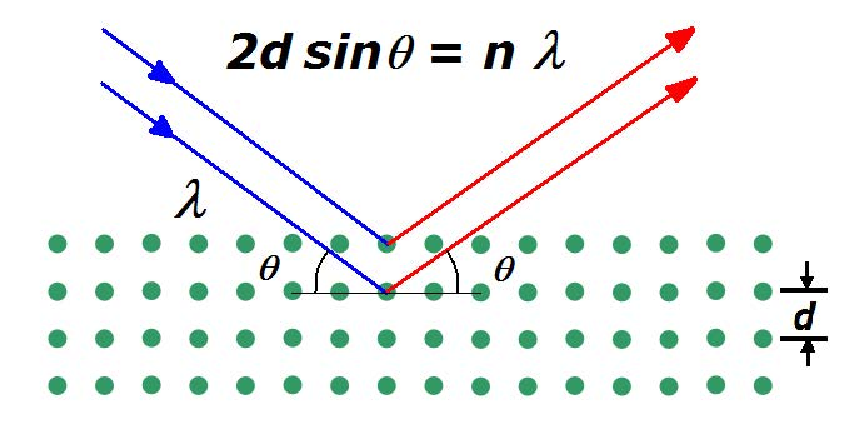
\includegraphics[width=10cm]{Bragglaw}
% \end{center}
% \caption[Braggov uklon.]{Braggov uklon je uklon oziroma sipanje 
% rentgenskih "zarkov na kristalni mre"zi. Pri tem pride v dolo"cenih 
% smereh zaradi interference do mo"cnih oja"canj. 
% Slika je povzeta iz \cite{Bragg}.}
% \label{pic1}
% \end{figure}

\index{plovke}



\newpage
\section{Formati slik}

% V \LaTeX{}ov dokument lahko vklju"cimo slike razli"cnih formatov. 
% Vedeti pa moramo, da program {\tt pdflatex} podpira ve"c formatov 
% kot {\tt latex}. Pri uporabi programa {\tt latex} lahko vstavljamo 
% slike edino v formatu PostScript (.ps ali .eps --- kon"cnica ni
% va"zna, le slika mora imeti definiran okvir, ki je zapisan
% v njeni datoteki, obi"cajno v formatu \%\%{\tt BoundingBox x1 y1 x2 y2}). 
% "Ce uporabljamo {\tt pdflatex}, so primerni formati na primer 
% .png, .pdf in .jpg.  Tudi slike v formatu .eps je mo"zno vstaviti,
% "ce tako kot v tem vzorcu uporabimo paket {\tt epstopdf}, ki vsako
% .eps sliko samodejno pretvori v obliko .pdf.  (Lahko pa seveda
% vsako .ps in .eps sliko "ze prej sami pretvorimo v sliko formata .pdf
% z istim programom in uporabljamo le .pdf slike.  To je morda
% celo najbolj priporo"cljiva pot.)  Strnjeno v Tabeli~\ref{tbl1}.




\chapter{Zaključek}

P

%%% LITERATURA

\cleardoublepage\phantomsection
\addcontentsline{toc}{chapter}{Literatura}
\bibliographystyle{myapsrevSLO}
\bibliography{Bibliografija}

%%% DODATKI

\cleardoublepage
\renewcommand\appendixname{Dodatek}
\begin{appendices}

\chapter{Naslov prvega dodatka}
    

\chapter{Naslov drugega dodatka}

\end{appendices}

%%% KAZALO (NEOBVEZNO)

\cleardoublepage
\printindex

\end{document}